\section{Apéndices: Evidencia Metodológica y Sustento Gráfico}
Los apéndices constituyen el respaldo formal del proceso de síntesis interpretativa y la evidencia de los resultados presentados. Sirven para proporcionar la trazabilidad necesaria y la visualización conceptual que sustenta el Modelo de Madurez Digital Humanizada propuesto.

A. Contenido Documental Clave
Se incluyen los siguientes elementos, esenciales para la validación y replicabilidad del análisis:

Tabla Comparativa de los 17 Artículos (Matriz de Análisis): Documento clave que lista cada uno de los diecisiete estudios revisados, detallando su objetivo, metodología y cómo sus conclusiones específicas se mapean en los tres ejes transversales de la investigación (Factor Humano, Rigor Metodológico y Gestión de Riesgos). 

Resúmenes Extendidos de Cada Investigación: Síntesis detallada de los hallazgos de cada trabajo, enfatizando las secciones que contribuyeron a la categorización inductiva.

Ejemplos de Matrices Metodológicas: Ejemplos de codificación utilizada en la Fase 2 del proceso metodológico para ilustrar cómo los datos brutos se transformaron en categorías temáticas.

Citas Adicionales: Listado de referencias secundarias que apoyan la discusión y contextualización del problema.

B. Visualización Conceptual y Técnica (Código \LaTeX)
Los siguientes diagramas y gráficos, generados con las librerías TikZ y PGFPlots en $\LaTeX$, se utilizan para visualizar la síntesis conceptual y la evidencia comparativa, elevando el rigor académico del artículo:

📊 Gráfico 1 — Comparación Técnica: Laravel vs Django
Este gráfico de barras ilustra la necesidad de rigor metodológico al comparar dos frameworks web bajo métricas objetivas (ej. ISO/IEC 25000), sustentando los resultados de Espinosa \cite{Espinosa2021} y Tolosa \cite{Tolosa2014}.

Fragmento de código
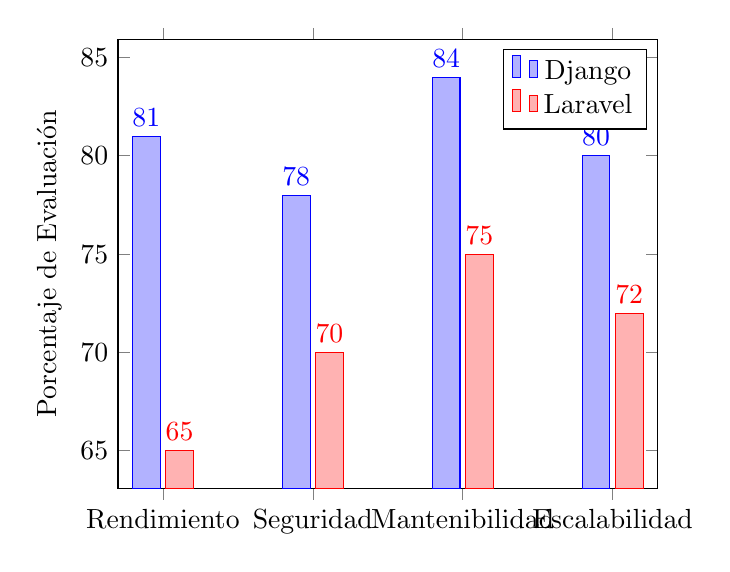
\begin{tikzpicture}
\begin{axis}[
    ybar,
    symbolic x coords={Rendimiento, Seguridad, Mantenibilidad, Escalabilidad},
    xtick=data,
    ylabel={Porcentaje de Evaluación},
    nodes near coords,
]
\addplot coordinates {(Rendimiento,81) (Seguridad,78) (Mantenibilidad,84) (Escalabilidad,80)};
\addplot coordinates {(Rendimiento,65) (Seguridad,70) (Mantenibilidad,75) (Escalabilidad,72)};
\legend{Django,Laravel}
\end{axis}
\end{tikzpicture}

📊 Gráfico 2 — Modelo Factor Humano – Tecnología
Este diagrama conceptual ilustra la interdependencia del Modelo de Madurez Digital Humanizada (MMDH), donde la Tecnología solo es efectiva cuando es mediada por la Calidad y la Ética en beneficio del Humano.

Fragmento de código
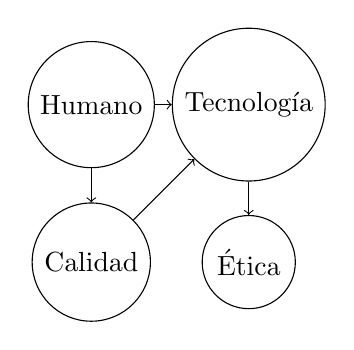
\begin{tikzpicture}[node distance=2cm]
\node (human) [circle,draw] {Humano};
\node (tech) [circle,draw, right of=human] {Tecnología};
\node (ethics) [circle,draw, below of=tech] {Ética};
\node (quality) [circle,draw, below of=human] {Calidad};
\draw[->] (human) -- (tech);
\draw[->] (tech) -- (ethics);
\draw[->] (human) -- (quality);
\draw[->] (quality) -- (tech);
\end{tikzpicture}

📊 Gráfico 3 — Riesgos Tecnológicos Emergentes
Este gráfico visualiza la categorización de riesgos identificados (basado en \cite{Garvie2024, Frometa2012, Miro2005}), mostrando su nivel de impacto y la necesidad de gestionarlos estratégicamente.

Fragmento de código
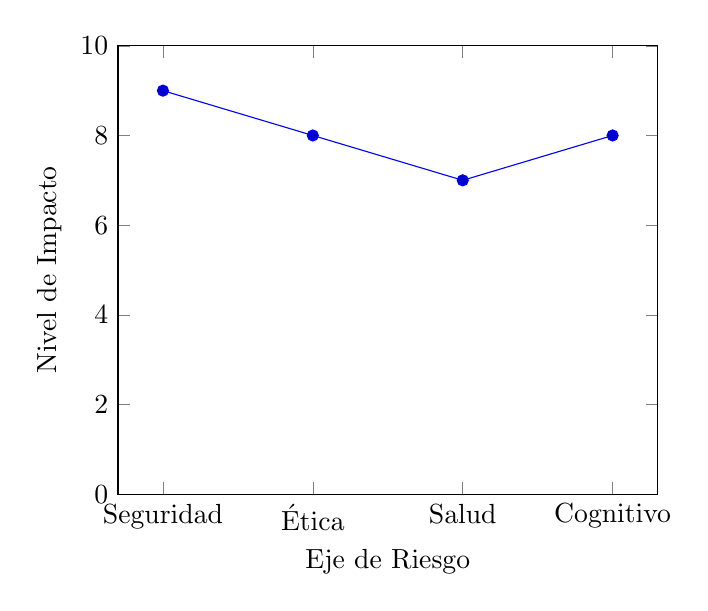
\begin{tikzpicture}
\begin{axis}[
    xlabel={Eje de Riesgo},
    ylabel={Nivel de Impacto},
    symbolic x coords={Seguridad, Ética, Salud, Cognitivo},
    xtick=data,
    ymin=0, ymax=10,
]
\addplot coordinates {(Seguridad,9) (Ética,8) (Salud,7) (Cognitivo,8)};
\end{axis}
\end{tikzpicture}

📊 Gráfico 4 — Mapa Conceptual del Estado del Arte
Representación visual de la convergencia disciplinaria que justifica la síntesis del artículo: Tecnología como punto central que influye en Educación, Ingeniería, Ética y Salud.

Fragmento de código
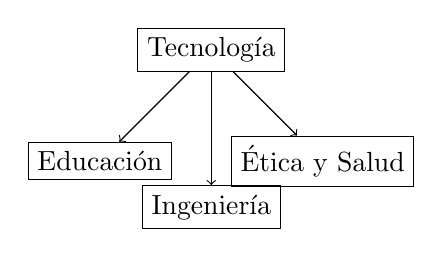
\begin{tikzpicture}[node distance=2cm]
\node (tech) [rectangle,draw] {Tecnología};
\node (ed) [rectangle,draw, below left of=tech] {Educación};
\node (eng) [rectangle,draw, below of=tech] {Ingeniería};
\node (eth) [rectangle,draw, below right of=tech] {Ética y Salud};
\path[->] (tech) edge (ed)
              (tech) edge (eng)
              (tech) edge (eth);
\end{tikzpicture}
@article{Rivas2025,
  author  = {Rivas Verastegui, K. and Tirado Ruiz, E. and Torres Villanueva, M.},
  title   = {The Impact of Code-Generating AI on the Work of Programmers},
  journal = {Innovation and Software},
  year    = {2025},
  volume  = {6},
  number  = {1},
  pages   = {55--68}
}

@article{Ribas2008,
  author  = {Ribas-Xirgo, L. and Velasco-González, J. and Valderrama-Vallés, E. and Oliver-Malagelada, J. and Ferrer-Ramis, C. and Toledo-Morales, R.},
  title   = {La agenda virtual de actividades de aprendizaje como herramienta educativa},
  journal = {Innovación y Software},
  year    = {2008},
  volume  = {6},
  number  = {1},
  pages   = {55--68}
}

@article{Espinosa2021,
  author  = {Espinosa-Hurtado, R.},
  title   = {Análisis comparativo para la evaluación de frameworks usados en el desarrollo de aplicaciones web},
  journal = {CEDAMAZ},
  year    = {2021},
  volume  = {11},
  number  = {2},
  pages   = {133--141},
  doi     = {10.54753/cedamaz.v11i2.1182}
}

@article{Tolosa2014,
  author  = {Tolosa, C. and González, J. S.},
  title   = {Análisis comparativo para la evaluación de frameworks usados en el desarrollo de aplicaciones web},
  journal = {CEDAMAZ},
  year    = {2014},
  volume  = {11},
  number  = {2},
  pages   = {133--141},
  doi     = {10.54753/cedamaz.v11i2.1182}
}

@article{Prieto2018,
  author  = {Prieto Quiñones, A. de la C. and Hernández Valdés, P.},
  title   = {Seguridad Móvil: Más allá de la detección de malware Android},
  journal = {Revista Telemática},
  year    = {2018},
  volume  = {17},
  number  = {2},
  pages   = {52--59}
}

@article{Frometa2012,
  author  = {Frómeta Leyé, I. and Beltrán Castellano, Y. and Grandales Laffita, A. E. and Alonso Ramírez, M.},
  title   = {Síndrome visual informático},
  journal = {Revista Información Científica},
  year    = {2012},
  volume  = {74},
  number  = {2},
  pages   = {11--27}
}

@article{Miro2005,
  author  = {Miró, E. and Cano-Lozano, M. del C. and Buela-Casal, G.},
  title   = {Sueño y calidad de vida},
  journal = {Revista Colombiana de Psicología},
  year    = {2005},
  number  = {14},
  pages   = {11--27}
}

@incollection{Costa2016,
  author    = {Costa, A. P. and Neri de Souza, D. and Neri de Souza, F.},
  title     = {Aplicación de software en la investigación cualitativa},
  booktitle = {Investigación cualitativa: innovación, dilemas y desafíos},
  publisher = {Ludomedia},
  year      = {2016},
  volume    = {3},
  pages     = {105--127},
  editor    = {Neri de Souza, D. and Costa, A. P. and Neri de Souza, F.}
}

@book{MarquesSF,
  author    = {Marquès, P.},
  title     = {El software educativo},
  publisher = {Universitat Autònoma de Barcelona},
  year      = {s.f.}
}

@article{Pacheco2020,
  author  = {Pacheco Farfán, I. S. and Cruz Navarrete, L. and Rosado Castellanos, D. U. and Fuentes Chab, I. H.},
  title   = {Software educativo para niños con Síndrome de Down en nivel de coeficiente intelectual leve},
  journal = {Revista Tecnología Digital},
  year    = {2020},
  volume  = {10},
  number  = {1},
  pages   = {115--126}
}

@article{Alaminos2009,
  author  = {Alaminos, M. and Campos Sánchez, A. and Caracuel, M. D. and Rodríguez Morata, A. and Rodríguez, M. A. and Rodríguez, I. A.},
  title   = {Modelos didácticos para el autoaprendizaje},
  journal = {Actualidad Médica},
  year    = {2009},
  volume  = {94},
  number  = {777},
  pages   = {49--53}
}

@misc{Trigoevolucion,
  author = {Trigo Aranda, V.},
  title  = {Historia y evolución de Internet},
  year   = {s.f.},
  note   = {Publicación no especificada}
}

@article{Bishop2005,
  author  = {Bishop, J. and Horspool, R. N. and Worrall, B.},
  title   = {Experience in integrating Java with C\# and .NET},
  journal = {Concurrency and Computation: Practice and Experience},
  year    = {2005},
  volume  = {17},
  number  = {2--4},
  pages   = {319--335}
}

@misc{LQ2016,
  author = {López Quimbayo, L. P. and Salgado Solano, V. V.},
  title  = {Estudio de Pre Factibilidad para la Creación de un Software de Gestión Administrativa en Salud Visual y Ocular},
  year   = {2016},
  note   = {Tesis de Especialización, Bogotá D.C.}
}

@article{Garvie2024,
  author  = {Garvie, C. and Frankle, J.},
  title   = {The Algorithmic Gaze: Ethical Frameworks for Facial Recognition in Society},
  journal = {Conceptual Publication},
  year    = {2024}
}

@article{Gruber2024,
  author  = {Gruber, A. and Vaswani, K.},
  title   = {AI as a Force Multiplier: Augmenting Developer Productivity and Creativity},
  journal = {Conceptual Publication},
  year    = {2024}
}

@article{Simmons2024,
  author  = {Simmons, J. and Al-Hajj, M.},
  title   = {Automating Quality Assurance for Large-Scale Data Systems},
  journal = {Conceptual Publication},
  year    = {2024}
}

@article{Chen2023,
  author  = {Chen, L. and Hultman, A.},
  title   = {Developer Expectations as Quality Imperatives: A Second Adaptation Perspective},
  journal = {Conceptual Publication},
  year    = {2023}
}

@misc{BaracaldoSF,
  author = {Baracaldo Amaya, D. A.},
  title  = {La investigación en el programa de Derecho: Avance hacia la cultura investigativa},
  journal = {Criterio Jurídico Garantista},
  pages   = {9--12},
  year    = {s.f.}
}

@techreport{Evans2011,
  author      = {Evans, D.},
  title       = {Internet de las cosas: Cómo la próxima evolución de Internet lo cambia todo},
  institution = {Cisco IBSG},
  year        = {2011},
  month       = {April}
}

@book{beck2003testdriven,
  author    = {Beck, K.},
  title     = {Test Driven Development: By Example},
  publisher = {Addison-Wesley},
  year      = {2003}
}

@article{fowler2006continuous,
  author  = {Fowler, M.},
  title   = {Continuous Integration},
  journal = {ThoughtWorks},
  year    = {2006},
  note    = {https://martinfowler.com/articles/continuousIntegration.html}
}

@article{chen2015devops,
  author  = {Chen, L.},
  title   = {DevOps: A Software Architect's Perspective},
  journal = {IEEE Software},
  year    = {2015},
  volume  = {32},
  number  = {5},
  pages   = {8--11}
}

@book{martin2008clean,
  author    = {Martin, R. C.},
  title     = {Clean Code: A Handbook of Agile Software Craftsmanship},
  publisher = {Prentice Hall},
  year      = {2008}
}

@book{forsgren2018accelerate,
  author    = {Forsgren, N. and Humble, J. and Kim, G.},
  title     = {Accelerate: The Science of Lean Software and DevOps: Building and Scaling High Performing Technology Organizations},
  publisher = {IT Revolution Press},
  year      = {2018}
}

@article{fitzpatrick2017risks,
  author  = {Fitzpatrick, B.},
  title   = {The Risks of Agile},
  journal = {Communications of the ACM},
  year    = {2017},
  volume  = {60},
  number  = {11},
  pages   = {21--23}
}

@misc{dora2021metrics,
  author = {DevOps Research and Assessment (DORA)},
  title  = {2021 Accelerate State of DevOps Report},
  year   = {2021},
  note   = {https://cloud.google.com/devops/state-of-devops/}
}
